\documentclass{article}
\usepackage{amsfonts}
\usepackage{amssymb}
\usepackage{graphicx}
\usepackage{amsmath} % import  amsmath to use align 
\usepackage{hyperref} % for inserting url

\begin{document}
  \title{復習機能付きの英中辞書}
  \author{王志軍}
  \maketitle
  
Hello \textbf{world}, \textit{here} is my \texttt{first} document!
% This is a comment
This is not a comment

\begin{enumerate}
\item[2.] This is an item
\item[3.] This is another item
  \begin{enumerate}
    \item here is a subpart
    \item here is another subpart
  \end{enumerate}
\item[4.] This is the third item.\\ \\
\end{enumerate}

Here is some math $x^2$ and $y_k$ \\ \\
This is some more advanced subscripts and superscripts \\ \\
$x^{123}$ and $y_{ijk}$. \\ \\
Let's mix and match $x^{2_i}$ or $x^{123}_{xyz}$  \\ \\

% align* for no equation 
% align for equation
\begin{align} 
% & means "line up here"
0 &= 3x^3+3x^2-6x \\  
&= 3( x^3 + x^2 - 2x) \\
&= 3x(x^2 + x -2) \\
&=3x(x+2)(x-1) \\
& \therefore \\
x &= 0, -2, 1 \\ \\
\end{align} \\ \\
Here some different matrices.\\ \\
bmatrix
$
\begin{bmatrix}
  1 & 2 & 3 \\
  a & b & 3 \\
\end{bmatrix}
$ \\ \\
pmatrix
$
\begin{pmatrix}
  1 & 2 & 3 & 4 & 5 \\
  a & b & 3 & d & e \\
\end{pmatrix}
$ \\ \\
Here is a fraction $\frac{x^2}{x^3} = \frac{1}{x}$ \\
Here is a \textbf{another }fraction $\dfrac{x^2}{x^3} = \dfrac{1}{x}$ \\ \\
Here is a squre root $\sqrt{16} = 4$ \\ \\
Here is a integral $\int_{a}^{b}f(x)dx$ \\ \\
$x = \frac{-b \pm \sqrt{b^2-4ac}}{2a}$ \\ \\
% Use verbatim environment to insert code
\begin{verbatim}
#!/usr/bin/env python
import os
if True:
    print os.path
\end{verbatim}
\begin{figure}[ht!]
\centering
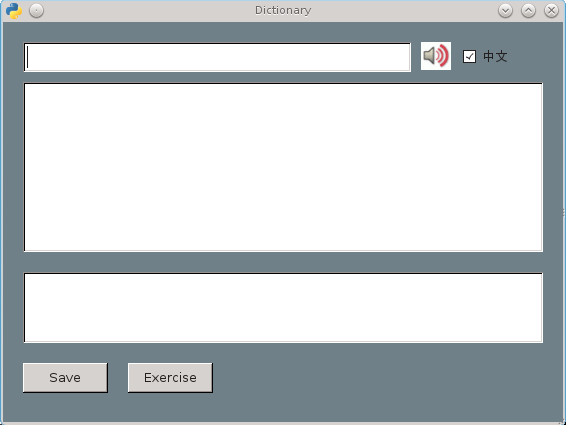
\includegraphics[width=45mm]{main.png}
\caption{A simple caption}
\label{overflow}
\end{figure}
\href{http://stackoverflow.com/questions/3134187/how-to-add-a-jpg-image-in-latex}{How to add image to LaTeX} \\
\begin{table}
\centering
  \begin{tabular}{|l|l|p{1cm}|}
\hline
  h1 & h2 & h3 \\
\hline
  a  & b  & This is the size of my column \\
\hline
  \end{tabular}
\end{table}
\end{document}

